\chapter{Apéndice A: Esquemáticos}
\renewcommand{\thepage}{A-\arabic{page}}
\setcounter{page}{1}
    Este apéndice presenta los esquemáticos eléctricos desarrollados para el proyecto \textcolor{dark_violet}{\textbf{GraviCap}}. Los esquemáticos incluidos proporcionan una visión detallada de los circuitos clave que permiten el funcionamiento eficiente del sistema. Estos esquemáticos son fundamentales para comprender la implementación de los sistemas de control y gestión de energía, y sirven como guía técnica para la construcción y funcionamiento del prototipo.
    Los dos esquemáticos que se incluyen en este apéndice son:\par
    
    \begin{itemize} [label = ]
    \setlength{\itemindent}{2em}
    
        \item MPPT (Maximum Power Point Tracking): Este esquema muestra el diseño del sistema encargado de optimizar la recolección de energía desde los paneles solares, asegurando que el sistema opere en el punto de máxima eficiencia, maximizando la energía capturada y transferida a la batería.\par
        \item Sistema de Control: Este esquema describe el hardware y la lógica de control del sistema de batería gravitatoria, incluyendo los componentes encargados de gestionar el flujo de energía entre la batería y la carga, así como los sensores que permiten un control preciso del sistema.\par
    \end{itemize}
    
    Ambos esquemáticos son esenciales para el correcto funcionamiento del sistema y proporcionan las bases técnicas para futuras expansiones o modificaciones en el diseño.\par

    \begin{landscape}
        \begin{sidewaysfigure}
            \centering
            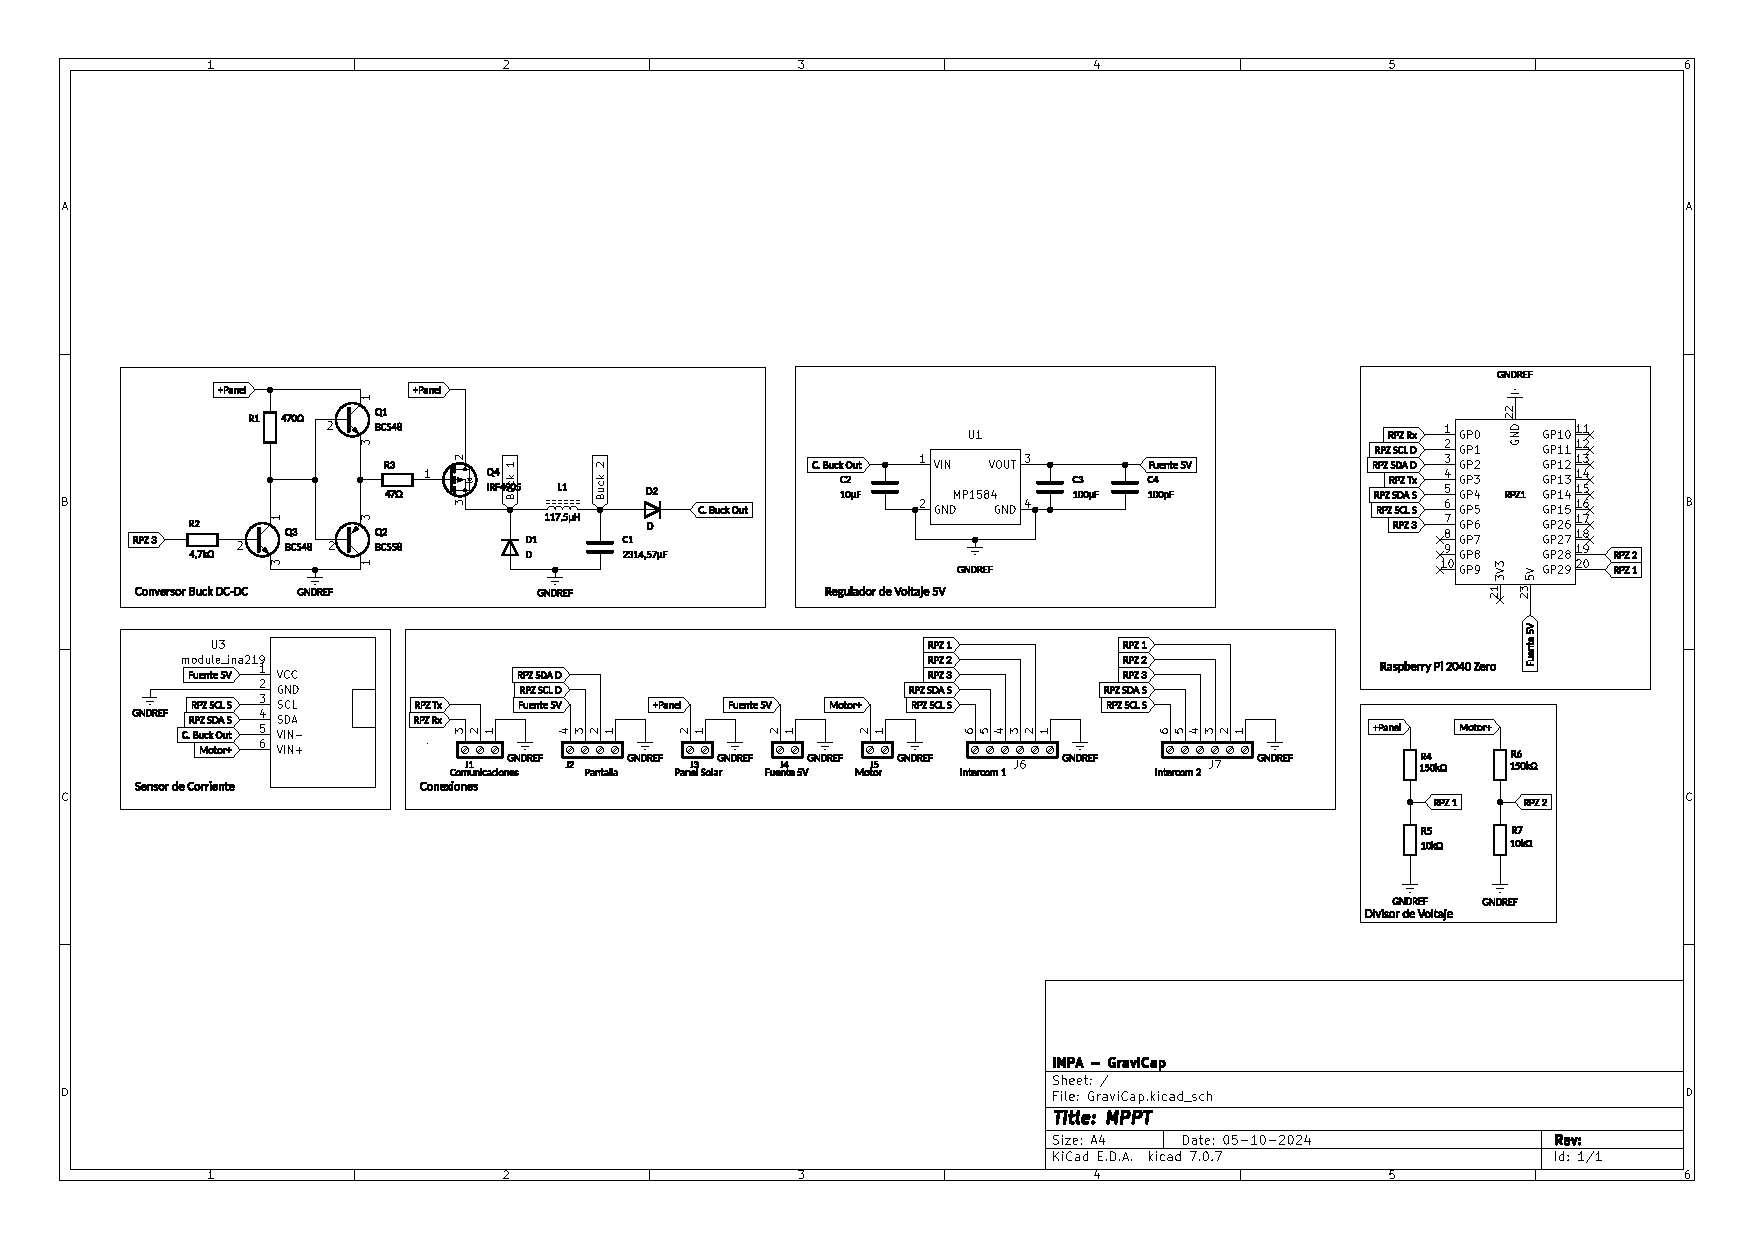
\includegraphics[angle=270, width=\textwidth,height=\textheight,keepaspectratio]{Imagenes/Anexo_A/Esquemático - MPPT.pdf}
            \label{fig:A_1}
        \end{sidewaysfigure}
        
        \newpage

        \begin{sidewaysfigure}
            \centering
            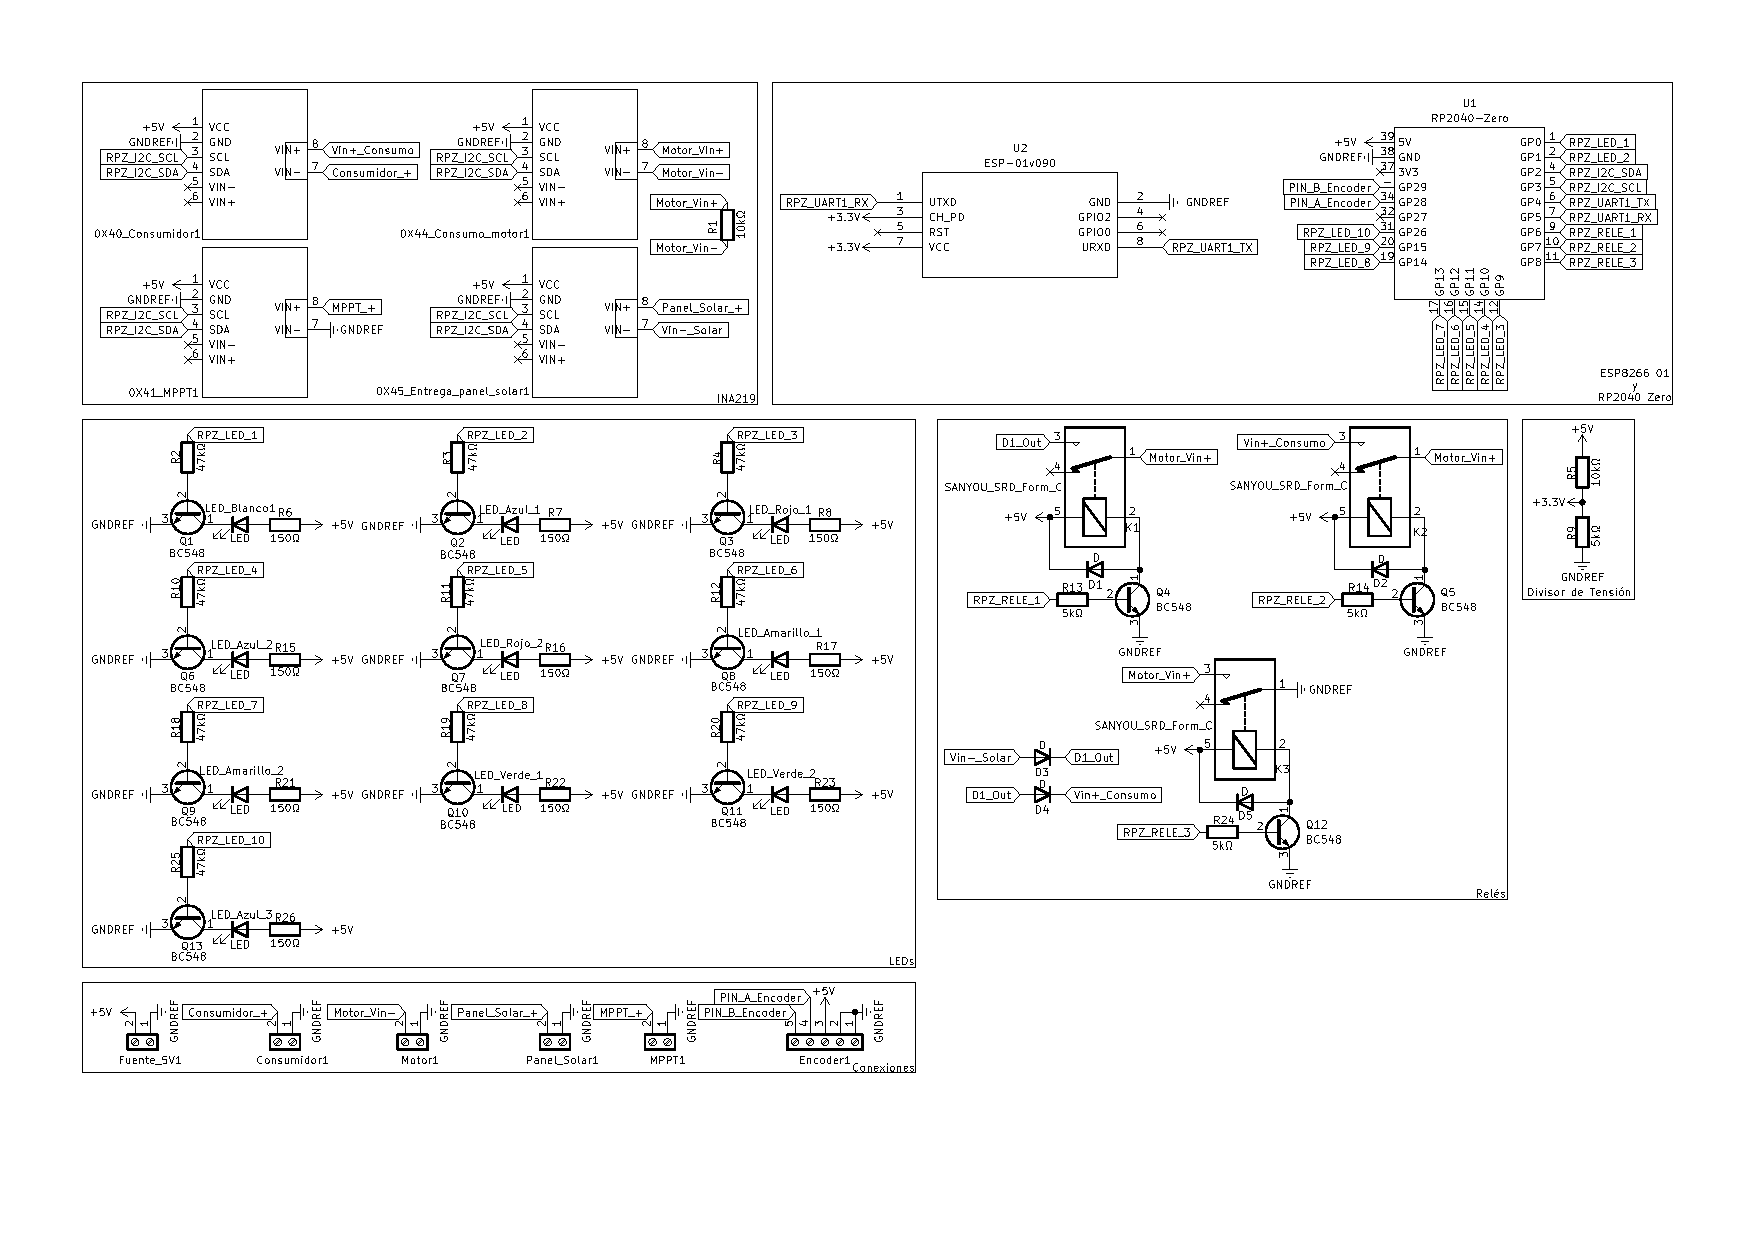
\includegraphics[angle=270, width=\textwidth,height=\textheight,keepaspectratio]{Imagenes/Anexo_A/Esquemático - Etapa_de_Control.pdf}
            \label{fig:A_2}
        \end{sidewaysfigure}

        \newpage

        \begin{sidewaysfigure}
            \centering
            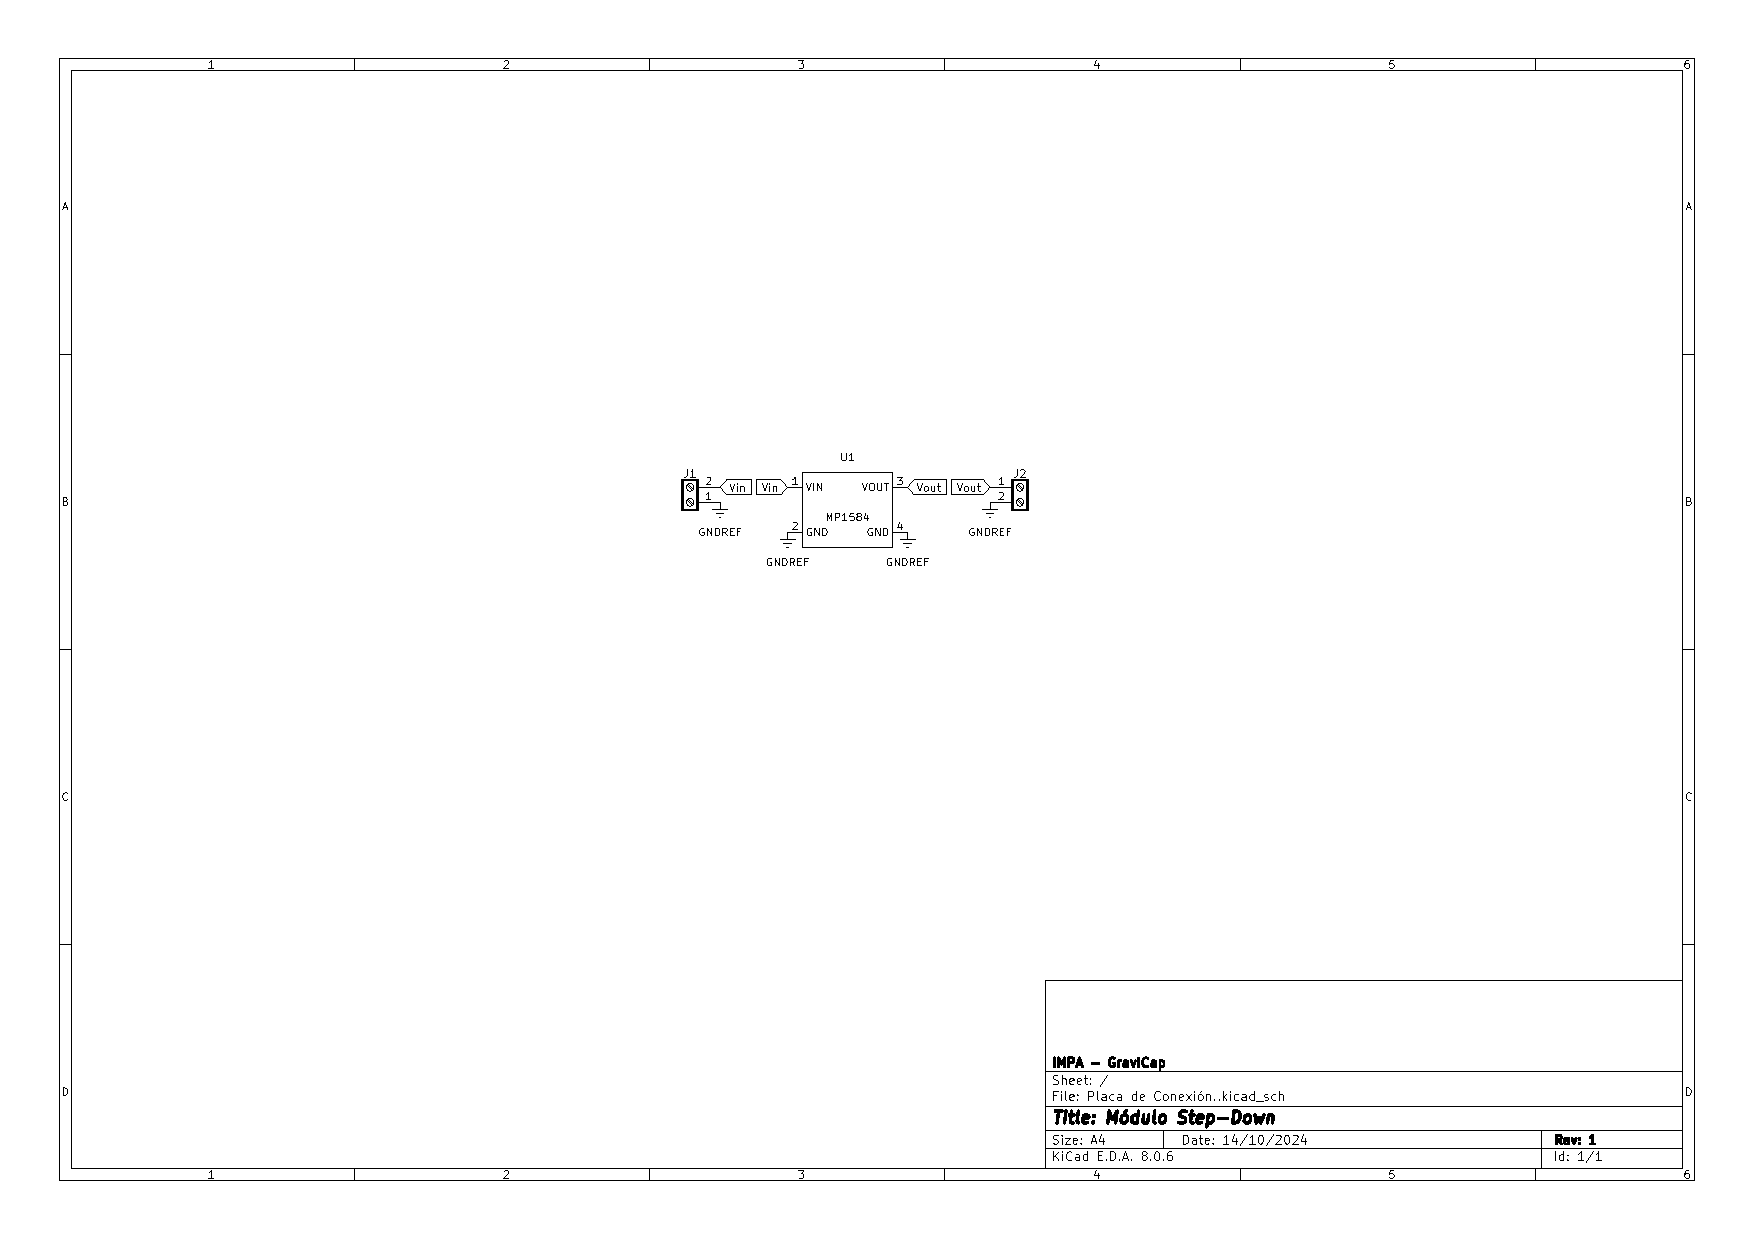
\includegraphics[angle=270, width=\textwidth,height=\textheight,keepaspectratio]{Imagenes/Anexo_A/Esquemático - Placa_de_Conexion.pdf}
            \label{fig:A_3}
        \end{sidewaysfigure}
        
    \end{landscape}